\chapter{The polaron problem} \label{ch:polarons}

In this chapter, we describe and compare different models that have been proposed for the description of polarons. We start by reviewing the Landau-Pekar model, the first to be proposed and the simplest one. Then, Fröhlich and Holstein models are discussed as well. These two models are currently used for the description of large and small polarons, respectively. A comparison of the properties of small and large polarons is presented in the last section.

\section{Landau-Pekar model} \label{sec:landau_pekar}
In the Landau-Pekar model, the electron is described by a wavefunction $\Psi(\vec{r})$ moving in a dielectric continuum medium. The static potential of the crystal is taken into account associating at the electron an effective mass $m^*$ (see \Cref{sec:electrons}). If we allow the medium to be polarized, the energy of the system is given by the kinetic energy of electron plus the energy of the electromagnetic field
\begin{equation} \label{eq:energy_landau}
    E = \frac{\hslash^2}{2m^*} \int \differential\vec{r} |\grad \psi(\vec{r})|^2 + \oh \int \differential \vec{r} \vec{E}\cdot \vec{D}
\end{equation}
$\vec{D}$ can be expressed, using the Gauss law, as $\div\vec{D} = \rho = -e |\rr{\psi}|^2$, or equivalently
\begin{equation}
    \vec{D} = -\frac{e}{4\pi} \grad \int \differential \vec{r}' \frac{|\psi(\vec{r})|^2}{|\vec{r}-\vec{r}'|}
\end{equation}
Remembering that for a dielectric medium $\vec{D} = \varepsilon_0 \epsilon^0 \vec{E}$, where $\varepsilon_0$ is the vacuum permittivity and $\epsilon^0$ is the static dielectric constant, we obtain for the electrostatic energy
\begin{equation} \label{eq:electric_energy_e0}
    \oh \int \differential \vec{r}  \vec{E}\cdot \vec{D} =
    \oh \frac{1}{4\pi\varepsilon_0} \frac{e^2}{\epsilon^0} \int \differential \vec{r} \differential \vec{r}' \frac{|\psi(\vec{r})|^2|\psi(\vec{r}')|^2}{|\vec{r}-\vec{r}'|}
\end{equation}
In the previous expression, $\vec{E}$ includes contributions from both the displacement of the ions and the electric screening of the electrons. The latter effect is already taken into account by the effective mass in the expression of the kinetic energy, so we have to remove its contribution. Since the ions have a much larger mass than the electrons, they will not contribute to the high-frequency dielectric constant $\epsilon^\infty$. Thus, $\epsilon^\infty$ expresses the contribution of electrons to the total dielectric constant. Subtracting it in the previous expression, we obtain
\begin{equation}
    \oh \int \differential \vec{r} \vec{E}\cdot \vec{D} =
    \oh \frac{e^2}{4\pi\varepsilon_0} \left( \frac{1}{\epsilon^0} - \frac{1}{\epsilon^\infty} \right) \int \differential \vec{r} \differential \vec{r}' \frac{|\psi(\vec{r})|^2|\psi(\vec{r}')|^2}{|\vec{r}-\vec{r}'|}
\end{equation}
If we define $1/\kappa = 1/\epsilon^\infty - 1/\epsilon^0$, we can rewrite the total energy as a functional of $\psi$
\begin{equation}
    E[\psi] = \frac{\hslash^2}{2m^*} \int \differential\vec{r} |\grad \psi(\vec{r})|^2 - \oh \frac{e^2}{4\pi\varepsilon_0} \frac{1}{\kappa} \int \differential \vec{r} \differential \vec{r}' \frac{|\psi(\vec{r})|^2|\psi(\vec{r}')|^2}{|\vec{r}-\vec{r}'|}
\end{equation}
Following a variational approach, this functional can be minimized to find the polaron ground state energy. To do so, we must include a normalization constraint. This is done with the help of a Lagrange multiplier $\varepsilon$
\begin{multline} \label{eq:landau_variational_energy}
    E[\psi, \varepsilon] = \frac{\hslash^2}{2m^*} \int \differential\vec{r} |\grad \psi(\vec{r})|^2 - \oh \frac{e^2}{4\pi\varepsilon_0} \frac{1}{\kappa} \int \differential \vec{r}' \frac{|\psi(\vec{r})|^2|\psi(\vec{r}')|^2}{|\vec{r}-\vec{r}'|}
    \\ - \varepsilon \left( \int \differential\vec{r} |\psi(\vec{r})|^2 -1 \right)
\end{multline}
Minimizing with respect to $\psi^*$ and $\varepsilon$, we obtain a Schr\"{o}dinger-type equation
\begin{equation} \label{eq:landau_schr_eq}
    \left(-\frac{\hslash^2}{2m^*} \laplacian - \frac{e^2}{4\pi\varepsilon_0} \frac{1}{\kappa} \int \differential \vec{r}' \frac{\psi(\vec{r}')|^2}{|\vec{r}-\vec{r}'|} \right) \psi(\vec{r}) = \varepsilon \psi(\vec{r})
\end{equation}
The Lagrange multiplier $\varepsilon$ has the dimension of an energy, but it not exactly the polaron ground state energy. Projecting \cref{eq:landau_schr_eq} onto $\psi^*$ and confronting the result with \cref{eq:landau_variational_energy}, we obtain a ground state energy $E_0$
\begin{equation}
    E_0 = \varepsilon + \oh \frac{e^2}{4\pi\varepsilon_0} \frac{1}{\kappa} \int \differential \vec{r}' \frac{|\psi(\vec{r})|^2|\psi(\vec{r}')|^2}{|\vec{r}-\vec{r}'|}
\end{equation}

\Cref{eq:landau_schr_eq} is not known to have an exact solution. However, given the similarity with the hydrogen atom Hamiltonian, we can use as a trial wavefunction $(\pi r_p^3)^{-1/2} e^{-r/r_p}$ and minimize $E$ with respect to $r_p$. As in the hydrogen atom, the kinetic term minimization favours larger $r_p$ (delocalized states) and the potential term favours smaller $r_p$ (localized states). Performing the minimization \cite{alexandrov2010}, $r_p$ is found to be
\begin{equation}
    r_p = \frac{16}{5} \frac{\kappa}{m^*/m_e} a_0
\end{equation}
where $m_e$ is the mass of the electron and $a_0$ the Bohr radius. The value of the ground state energy is
\begin{equation}
    E_0 = -\frac{50}{512} \alpha^2 \hslash \omega_\text{LO}
\end{equation}
where $\omega_\text{LO}$ is the characteristic frequency of longitudinal optical phonon and
\begin{equation}
    \alpha = \frac{e^2}{4\pi\varepsilon_0\hslash} \sqrt{\frac{m^*}{2\hslash\omega_\text{LO}}} \frac{1}{\kappa}
\end{equation}

Despite its simplicity, the Landau-Pekar model provides simple formulas for the polaron ground state, radius and effective mass \cite{landau1948}. However, to have polaron bound states, $\kappa$ must be positive, which implies $\epsilon^0 > \epsilon^\infty$. This is true only for polar crystals, but polarons are observed in non-polar crystals as well. Moreover, this model carries an intrinsic contradiction. Treating the medium as a continuum requires the polaron to be large, but formally justified results can only be obtained in the strong coupling regime, a situation improbable for real materials.
\section{Fröhlich polarons}
We have anticipated in \cref{sec:landau_pekar} a simple model for the description of polarons. To improve that first model, we have to describe the mechanics of the lattice polarization more precisely. In this section, we discuss the Fröhlich Hamiltonian, derived by Fröhlich in 1950 \cite{frohlich1950}. This Hamiltonian is appropriate for the description of large polarons in ionic crystals and polar semiconductors. In these materials, we expect electrons to interact strongly with longitudinal optical phonons. The interaction is mediated by the electric field produced by the polarization of the lattice. The contribution of transversal phonons is expected to be negligible because of the smaller electric field they produce.

\subsection{Derivation of the Fröhlich Hamiltonian}
In this section we derive the Fröhlich Hamiltonian following the approach described by Kittel \cite{kittel1987}. We assume the longitudinal phonons to be dispersionless (with frequency $\omega_\text{LO}$) and we treat the polarizable medium as a continuum.

In an ionic crystal, the polarization $\vec{P}$ can be considered as the sum of two components: the optical polarization $\vec{P}_o$ and the infra-red polarization $\vec{P}_\text{ir}$. The former is due to the displacement of bound electrons, and it is characterized by a resonance frequency in the optical or ultraviolet region; the latter is due to the displacement of ions and its resonance frequency is in the infra-red region. Given the slow velocities of the electrons that we are going to consider, the optical polarization is always excited at its static value. Thus, given the absence of a dependence on the velocity of the electron, the optical polarization $\vec{P}_o$ is of no interest to us, since it does not modify the energy of the electron between different states. On the other hand, this does not apply to the infra-red polarization, because of its lower resonance frequency. At long distances from the electric charge (placed at $\vec{r}_0)$, $\vec{P}_\text{ir}$ can be obtained subtracting the optical polarization $\vec{P}_o$ from the total polarization $\vec{P}$. Thus, it can be derived from an electric potential $V(\vec{r})$ by
\begin{equation} \label{eq:polarization_potential}
    4\pi\vec{P}_\text{ir}(\vec{r}) = \grad V(\vec{r})
\end{equation}
where
\begin{equation}
    V(\vec{r}) = -\frac{1}{\kappa} \frac{e}{|\vec{r}-\vec{r}_0|}
\end{equation}
with $1/\kappa = 1 / \epsilon^\infty - 1/\epsilon^0$. As in the Landau-Pekar model, the contribution of the lattice to the dielectric constant ($\kappa$) is obtained by removing the contribution of the electrons ($\epsilon^\infty$) from the static dielectric constant ($\epsilon^0$).


The infra-red polarization is proportional to the amplitude of the displacement of the ions. Generalizing \cref{eq:phonon_coordinates}, for a generic point $\vec{r}$, we can express the displacement in the point $\vec{r}$ as
\begin{equation}
    \vec{\xi}(\vec{r}) = \sum_{\vec{q}} A \vers{\epsilon}_{\vec{q}} e^{i\vec{q} \cdot \vec{r}} (\oper{b}_{\vec{q}} + \adjop{b}_{-\vec{q}})
\end{equation}
where we have dropped the indices $a$ and $\lambda$ because we are considering atoms of the same mass and phonons of the same branch. Moreover, $A$ does not depend on $\vec{q}$ because the phonons are assumed to be dispersionless. Since we are considering only longitudinal phonons, the polarization vector $\vers{\epsilon}_{\vec{q}}$ must be parallel to $\vec{q}$. However, we cannot simply suppose $\vers{\epsilon}_{\vec{q}} = \vers{q}$. In fact, we have to guarantee that $\vec{\xi}(\vec{r})$ is real:
\begin{equation}
    \vec{\xi}^\dagger(\vec{r}) = \sum_{\vec{q}} A \vers{\epsilon}_{\vec{q}}^\dagger e^{-i\vec{q} \cdot \vec{r}} (\adjop{b}_{\vec{q}} + \oper{b}_{-\vec{q}})
    = \sum_{\vec{q}} A \vers{\epsilon}_{-\vec{q}}^\dagger e^{i\vec{q} \cdot \vec{r}} (\oper{b}_{\vec{q}} + \adjop{b}_{-\vec{q}})
    = \vec{\xi}(\vec{r})
\end{equation}
This implies $\vers{\epsilon}_{\vec{q}}^\dagger = \vers{\epsilon}_{-\vec{q}}$, and then $\vers{\epsilon}_{\vec{q}} = i\vers{q}$.

As we anticipated, $\vec{P}_\text{ir}$ is proportional to the amplitude of the displacement
\begin{equation} \label{eq:polarization_field}
    \vec{P}_\text{ir} = F \vec{\xi}(\vec{r}) = i F \sum_{\vec{q}} A \vers{q} e^{i\vec{q} \cdot \vec{r}} (\oper{b}_{\vec{q}} + \adjop{b}_{-\vec{q}})
\end{equation}
where F is a constant to be determined. We expand the electric potential in a Fourier series
\begin{equation}
    V(\vec{r}) = \sum_\vec{q} V(\vec{q}) e^{i\vec{q} \cdot \vec{r}}
\end{equation}
and we compute the gradient
\begin{equation} \label{eq:electric_field}
    \grad V(\vec{r}) = i \sum_\vec{q} \vec{q} V(\vec{q}) e^{i\vec{q} \cdot \vec{r}}
\end{equation}
Using \cref{eq:polarization_potential} and comparing \cref{eq:polarization_field} with \cref{eq:electric_field}, we find
\begin{equation}
    V(\vec{q}) = 4\pi \frac{F A}{q} (\oper{b}_{\vec{q}} + \adjop{b}_{-\vec{q}})
\end{equation}
We want to express the constant $F$ in terms of the interaction energy of two electrons in a polarizable material of dielectric constant $\epsilon$. We consider two electrons completely localized in two points $\vec{r}_1$ and $\vec{r}_2$. The electrons will interact directly through the vacuum electric field and indirectly through a perturbation induced by the optical phonon field. The interaction Hamiltonian is given by the sum of the potential of the two electrons
\begin{multline} \label{eq:hamiltonian_coulomb_medium}
    H_\text{el-el} = -e V(\vec{r}_1) -e V(\vec{r}_2)
    = 4\pi e F A \sum_\vec{q} q^{-1} (e^{i\vec{q} \cdot \vec{r}_1} + e^{i\vec{q} \cdot \vec{r}_2} ) (\oper{b}_{\vec{q}} + \adjop{b}_{-\vec{q}})
    \\ = 4\pi e F A \sum_\vec{q} q^{-1} \left[ \oper{b}_{\vec{q}} (e^{i\vec{q} \cdot \vec{r}_1} + e^{i\vec{q} \cdot \vec{r}_2} )   + \adjop{b}_{\vec{q}} (e^{-i\vec{q} \cdot \vec{r}_1} + e^{-i\vec{q} \cdot \vec{r}_2} )\right]
\end{multline}
where in the second line we have changed the sign of $\vec{q}$ in the second term, using the fact that the sum is taken over all $\vec{q}$. The second-order energy perturbation caused by the previous Hamiltonian is given by
\begin{equation}
    \Delta E = -\sum_\vec{q} \frac{\bra{0}H_\text{el-el}\ket{\vec{q}}\bra{\vec{q}}H_\text{el-el}\ket{0}}{\hslash\omega_\text{LO}}
\end{equation}
where $\ket{0}$ and $\ket{\vec{q}}$ are respectively states with no phonons and a single LO phonon in the state $\vec{q}$ with energy $\hslash\omega_\text{LO}$. Inserting \cref{eq:hamiltonian_coulomb_medium} in the previous expression and dropping the terms with $\vec{r}_1$ and $\vec{r}_2$ alone, which are self-energy terms,
\begin{multline}
    \Delta E = -2\sum_\vec{q} \frac{\bra{0}eV(\vec{r}_1)\ket{\vec{q}}\bra{\vec{q}}eV(\vec{r}_2)\ket{0}}{\hslash\omega_\text{LO}}
    \\ = -2 \frac{(4\pi eFA)^2}{\hslash \omega_\text{LO}} \sum_\vec{q} q^{-2} \bra{0}e^{i\vec{q}\cdot\vec{r}_1}(\oper{b}_{\vec{q}} + \adjop{b}_{\vec{q}})\ket{\vec{q}}\bra{\vec{q}}e^{-i\vec{q}\cdot\vec{r}_2}(\oper{b}_{\vec{q}} + \adjop{b}_{\vec{q}})\ket{0}
    \\ = - 2 \frac{(4\pi eFA)^2}{\hslash \omega_\text{LO}} \sum_\vec{q} q^{-2} \bra{\vec{q}}e^{i\vec{q}\cdot\vec{r}_1}\ket{\vec{q}}\bra{\vec{q}}e^{-i\vec{q}\cdot\vec{r}_2}\ket{\vec{q}}
    \\ = - 2 \frac{(4\pi eFA)^2}{\hslash \omega_\text{LO}} \sum_\vec{q}\frac{e^{i\vec{q}\cdot(\vec{r}_1 - \vec{r}_2)}}{q^2}
\end{multline}
Knowing that, when summed over all $\vec{q}$,
\begin{equation}
    \sum_\vec{q} \frac{4\pi}{q^2} e^{i\vec{q}\cdot \vec{r}} = \Omega \frac{1}{|\vec{r}|}
\end{equation}
where $\Omega$ is the volume of the region of interest, we can rewrite the perturbation energy as

\begin{equation}
    \Delta E = - \frac{8\pi \Omega A^2 F^2}{\hslash \omega_\text{LO}} \frac{e^2}{|\vec{r}_1 - \vec{r}_2|}
\end{equation}

The form of this interaction is exactly the same of an attractive Coulomb potential between two charges placed at $\vec{r}_1$ and $\vec{r}_2$. The origin of this attraction is the polarization of the ions of the medium. Thus, the factor
\begin{equation} \label{eq:dielectric_factor}
    - \frac{8\pi \Omega A^2 F^2}{\hslash \omega_\text{LO}}
\end{equation}
gives exactly the contribution of the ions to the dielectric constant. Since the static dielectric constant $\epsilon^0$ includes both the contribution of the ions and of the electrons, and the high-frequency dielectric constant $\epsilon^\infty$ only the contribution of the electrons, we can express \cref{eq:dielectric_factor} as
\begin{equation}
    \frac{1}{\epsilon^0} = \frac{1}{\epsilon^\infty} - \frac{8\pi \Omega A^2 F^2}{\hslash \omega_\text{LO}}
\end{equation}
The electric potential is then given by
\begin{equation}
    V(\vec{r}) = \sum_\vec{q} V(\vec{q}) e^{i\vec{q} \cdot \vec{r}}
    =  \sum_\vec{q} \left[ \frac{2\pi e^2 \hslash \omega_\text{LO}}{\Omega q^2} \left( \frac{1}{\epsilon^\infty} - \frac{1}{\epsilon^0} \right) \right]^{1/2} (\oper{b}_{\vec{q}} + \adjop{b}_{-\vec{q}}) e^{i\vec{q}\cdot\vec{r}}
\end{equation}
and writing it in a fully second-quantized form, we find
\begin{equation}
    \oper{H}_\text{el-ph} =  \sum_{\vec{k}'\vec{k}} \sum_{\vec{q}} \left[ \frac{2\pi e^2 \hslash \omega_\text{LO}}{\Omega q^2} \left( \frac{1}{\epsilon^\infty} - \frac{1}{\epsilon^0} \right) \right]^{1/2} \bra{\vec{k}'}e^{i\vec{q}\cdot\vec{r}}\ket{\vec{k}}(\oper{b}_{\vec{q}\lambda} + \adjop{b}_{-\vec{q}\lambda}) \adjop{c}_{\vec{k}'}\oper{c}_{\vec{k}}
\end{equation}
Confronting the previous expression with \cref{eq:general_electron_phonon_hamiltonian}, we can identify the interaction matrix
\begin{equation}
    M_{\vec{k}-\vec{q} \rightarrow \vec{k}} =  \left[ \frac{2\pi e^2 \hslash \omega_\text{LO}}{\Omega q^2} \left( \frac{1}{\epsilon^\infty} - \frac{1}{\epsilon^0} \right) \right]^{1/2}
\end{equation}
which is more commonly written as
\begin{equation} \label{eq:frohlich_matrix}
    M_\vec{q} =  \frac{\hslash \omega_\text{LO}}{|\vec{q}|} \left(\frac{\hslash}{2m\omega_\text{LO}}\right)^{1/4} \left(\frac{4\pi\alpha}{\Omega}\right)^{1/2}
\end{equation}
where $\alpha$ is the dimensionless Fröhlich coupling constant,  defined as
\begin{equation}
    \alpha = \frac{e^2}{\hslash} \left( \frac{1}{\epsilon^\infty} - \frac{1}{\epsilon^0} \right) \sqrt{\frac{m}{2\hslash\omega_\text{LO}}}
\end{equation}
where $m$ is the electron band mass.

Adding the electrons and phonons contributions, and approximating the wavefunctions of the electrons to plane waves as we did in \cref{eq:plane_waves}, we can write the Fröhlich Hamiltonian as
\begin{multline} \label{eq:frohlich_hamiltonian}
    H_\text{Fröhlich} = \sum_{\vec{k}} \frac{\hslash^2\vec{k}^2}{2m}
    + \sum_{\vec{q}} \hslash \omega_\text{LO} \left( \adjop{b}_{ \vec{q}} \oper{b}_{ \vec{q}} + \frac{1}{2} \right)
    \\ + \sum_{\vec{k}\vec{q}} \frac{\hslash \omega_\text{LO}}{|\vec{q}|} \left(\frac{\hslash}{2m\omega_\text{LO}}\right)^{1/4} \left(\frac{4\pi\alpha}{\Omega}\right)^{1/2} \adjop{c}_{\vec{k}}\oper{c}_{\vec{k}-\vec{q}} (\oper{b}_{\vec{q}} + \adjop{b}_{-\vec{q}})
\end{multline}
The interaction of the electrons with the lattice described by \cref{eq:frohlich_hamiltonian} has multiple effects. Some consequences we may expect are:
\begin{itemize}
    \item The electron band energy is decreased, because part of the energy is used to produce phonons.
    \item The effective mass of the electron is increased, because the electron has to deform the lattice while moving, carrying the deformation with itself.
    \item The mobility of the electron is modified, because the polaron experiences scattering effects different from the ones of a free electron.
\end{itemize}
We can analyse quantitatively the first of these two effects using approximation techniques. We will do it in the next two sections, applying perturbation theory and variational methods to the Fröhlich Hamiltonian.

\subsection{Weak coupling limit} \label{sec:weak_frohlich}
Polarons are often divided in two classes: large and small. The name is due to their effective radius $r_p$, which is defined as the effective radius of the polarized area. If $r_p$ is greater than the interatomic distance $l$, the polaron is said to be large; on the contrary, if $r_p \lesssim l$, the polaron is said to be small. In the former case, the coupling is usually weak ($\alpha < 1$), in the latter it is strong ($\alpha > 1$). In the weak-coupling regime, it is possible to use perturbation theory to derive some properties of large polarons.

The total Hamiltonian is
\begin{multline}
    \oper{H} = \oper{H}_\text{el} + \oper{H}_\text{ph} + \oper{H}_\text{el-ph}
    \\ = \sum_{\vec{k}} \frac{\hslash^2\vec{k}^2}{2m}
    + \sum_{\vec{q}} \hslash \omega_\text{LO} \left( \adjop{b}_{ \vec{q}} \oper{b}_{ \vec{q}} + \frac{1}{2} \right)
    + \sum_{\vec{k}\vec{q}} M_{\vec{q}}\adjop{c}_{\vec{k}}\oper{c}_{\vec{k}-\vec{q}} (\oper{b}_{\vec{q}} + \adjop{b}_{-\vec{q}})
\end{multline}
where $M_\vec{q}$ is given by \cref{eq:frohlich_matrix}
\begin{equation} \label{eq:frohlich_matrix_perturbation}
    M_\vec{q} =  \frac{\hslash \omega_\text{LO}}{|\vec{q}|} \left(\frac{\hslash}{2m\omega_\text{LO}}\right)^{1/4} \left(\frac{4\pi\alpha}{\Omega}\right)^{1/2}
\end{equation}
and it is supposed to be small ($\alpha < 1$). The unperturbed Hamiltonian
\begin{equation}
    \oper{H}^{(0)} = \oper{H}_\text{el} + \oper{H}_\text{ph}
\end{equation}
has plane waves $\ket{\vec{k}}$ as eigenfunctions of the single  electron part and many-body basis kets $\ket{n_1 \dots n_\vec{q} \dots}$ as eigenfunctions of the phonon part. The full eigenkets are given by the composition of the two parts $\ket{\vec{k}; \{n_\vec{q}\}} = \ket{\vec{k}}\ket{n_1 \dots n_\vec{q} \dots}$. The energy of this state is
\begin{equation}
    E_{\vec{k}, \{n_\vec{q}\}}^{(0)} = \frac{\hslash^2\vec{k}^2}{2m} + \hslash \omega_\text{LO}\sum n_\vec{q}
\end{equation}
and the ground state is given by an electron with $\vec{k}=0$ and the vacuum state $\ket{0}$ for the phonon part.
First-order perturbation theory results in no energy shift, since
\begin{equation}
    \bra{\vec{k}}\bra{0}(\oper{b}_{\vec{q}} + \adjop{b}_{-\vec{q}})\ket{0}\ket{\vec{k}} = 0
\end{equation}
Going to second order
\begin{equation}
    \Delta E_\vec{k}^{(2)} = \sum_{a\neq{\{\vec{k};0\}}} \frac{\left|\bra{\vec{k};0}\oper{H}_\text{el-ph}\ket{a}\right|^2}{E_{\{\vec{k};0\}} - E_a}
    = \sum_{a\neq{\{\vec{k};0\}}} \frac{\left|\bra{\vec{k};0} M_{\vec{q}}\adjop{c}_{\vec{k}}\oper{c}_{\vec{k}-\vec{q}} (\oper{b}_{\vec{q}} + \adjop{b}_{-\vec{q}})\ket{a}\right|^2}{E_{\{\vec{k};0\}} - E_a}
\end{equation}
where $\ket{a}$ is an excited state. The only states that contribute with non-null terms are states composed of an electron and a single phonon of wavevector $\vec{q}$. The electron is scattered by the phonon in a state of wavevector $\vec{k} - \vec{q}$, so that the total momentum is conserved. The kets $\ket{a}$ are thus of the form $\ket{\vec{k}-\vec{q}; n_\vec{q}=1}$, with energy
\begin{equation}
    E_a = \frac{\hslash^2}{2m}(\vec{k}-\vec{q})^2 + \hslash\omega_\text{LO}
    = \frac{\hslash^2\vec{k}^2}{2m} - \frac{\hslash^2\vec{k}\cdot\vec{q}}{m} + \frac{\hslash^2\vec{q}^2}{2m} + \hslash\omega_\text{LO}
\end{equation}
The shift in the energy is then
\begin{equation} \label{eq:delta_E_matrix}
    \Delta E_\vec{k} = -\sum_\vec{q} \frac{|M_\vec{q}|^2}{\hslash\omega_\text{LO} + \frac{\hslash^2}{2m}q^2 - \frac{\hslash^2}{m}\vec{k}\cdot\vec{q}}
\end{equation}
We may denote
\begin{equation} \label{eq:interaction_matrix_simplified}
    |M_\vec{q}|^2 = \frac{C}{q^2}
\end{equation}
where
\begin{equation} \label{eq:C}
    C = (\hslash \omega_\text{LO})^2 \left(\frac{\hslash}{2m\omega_\text{LO}}\right)^{1/2} \left(\frac{4\pi\alpha}{\Omega}\right)
\end{equation}
Defining $\mu = \frac{\vec{k}\cdot\vec{q}}{|\vec{k}||\vec{q}|}$, we can convert the sum in \cref{eq:delta_E_matrix} in an integral,
\begin{equation}
    \sum_\vec{q} \rightarrow \frac{\Omega}{(2\pi)^3} \int \differential\vec{q} = \frac{\Omega}{(2\pi)^3} \int 2\pi q^2 \differential q \differential \mu
\end{equation}
then,
\begin{equation}\label{eq:delta_E_integral}
    \Delta E_\vec{k} = - \frac{\Omega}{(2\pi)^2} \int_{-1}^1 \differential \mu \int_0^{q_\text{BZ}} \differential q \frac{C}{\hslash\omega_\text{LO} + \frac{\hslash^2}{2m}q^2 - \frac{\hslash^2}{m} kq\mu}
\end{equation}
where the integral is extended until the boundary of the first Brillouin zone. Although the integral in \cref{eq:delta_E_integral} may be exactly solved, we can gain some insights on the main physical meaning by developing it in powers of k and letting $q_\text{BZ} \rightarrow \infty$. Choosing an appropriate set of units, so that $\hslash  = \omega_\text{LO} = 2m = 1$,
\begin{equation}
    \Delta E_\vec{k} = - \frac{\alpha}{\pi} \left[
        2\int_0^\infty \differential q \frac{1}{1+q^2}
        + 4k^2 \int_{-1}^1 \differential \mu \int_0^\infty \differential q \frac{q^2\mu^2}{(1+q^2)^3} \right]
    = - \alpha - \frac{\alpha}{6}k^2
\end{equation}
and plugging back the standard units,
\begin{equation}
    \Delta E_\vec{k} = -\alpha \hslash \omega_\text{LO} - \frac{\alpha}{6}\frac{\hslash^2}{2m}k^2
\end{equation}
Finally, the perturbed energy is
\begin{equation} \label{eq:perturbation_energy}
    E_\vec{k} = -\alpha \hslash \omega_\text{LO} + \left(1 - \frac{\alpha}{6}\right)\frac{\hslash^2}{2m}k^2
\end{equation}
where the factor on the right can be interpreted as an electron with a new effective mass $m^* = m / (1-\alpha/6)$. The band energy is shifted down by an overall factor of $\alpha \hslash \omega_\text{LO}$ and the effective mass of the electron is increased. This is a reasonable conclusion: the electron digs itself a hole in the lattice potential, lowering its energy, and it has to carry the deformation along its path, resulting in a bigger effective mass.

It is also possible to compute the average number of phonons coupled with the electron at $T = \SI{0}{K}$. The phonon number operator is given by
\begin{equation}
    \oper{N}_\text{ph} = \sum_\vec{q} \adjop{b}_\vec{q} \oper{b}_\vec{q}
\end{equation}
so its average value is
\begin{equation} \label{eq:number_phonons_polaron}
    \langle \oper{N}_\text{ph} \rangle = \sum_\vec{q} \bra{\psi} \adjop{b}_\vec{q} \oper{b}_\vec{q} \ket{\psi}
\end{equation}
where $\ket{\psi}$ is the electron-phonon ket. The ket can be expanded near a state with no phonons $\ket{\vec{k}, 0}$
\begin{equation}
    \ket{\psi_\vec{k}} = \ket{\vec{k}, 0} + \ket{\delta\psi_\vec{k}}
\end{equation}
where $\ket{\delta\psi_\vec{k}}$ is the variation of the wavefunction due to the electron-phonons interaction. Using first-order perturbation theory, it can be found that
\begin{equation} \label{eq:sum_integral}
    \ket{\delta\psi_\vec{k}} = \sum_{a \neq \{\vec{k};0\}} \ket{a} \frac{\bra{\vec{k};0} \oper{H}_\text{el-ph} \ket{a}}{E_{\{\vec{k};0\}} - E_a}
    = \sum_\vec{q} \ket{\vec{k}-\vec{q};n_\vec{q}=1} \frac{M_\vec{q}}{E_{\{\vec{k};0\}} - E_{\{\vec{k}-\vec{q};n_\vec{q}=1\}}}
\end{equation}
Inserting the result in \cref{eq:number_phonons_polaron}, we obtain
\begin{equation}
    \langle \oper{N}_\text{ph} \rangle = \sum_\vec{q} \frac{\bra{\vec{k}-\vec{q};n_\vec{q}=1} \adjop{b}_\vec{q} \oper{b}_\vec{q} \ket{\vec{k}-\vec{q};n_\vec{q}=1}}{(\hslash\omega_\text{LO} + \frac{\hslash^2}{2m}q^2 - \frac{\hslash^2}{m}\vec{k}\cdot\vec{q})^2} |M_\vec{q}|^2
\end{equation}
and substituting $q$ and $\mu$ as before,
\begin{equation}
    \langle \oper{N}_\text{ph} \rangle = \sum_\vec{q} \frac{|M_\vec{q}|^2}{(\hslash\omega_\text{LO} + \frac{\hslash^2}{2m}q^2 - \frac{\hslash^2}{m} kq\mu)^2}
\end{equation}
or, expressed in our usual set of units,
\begin{equation}
    \langle \oper{N}_\text{ph} \rangle = \sum_\vec{q} \frac{|M_\vec{q}|^2}{(1 + q^2 - \frac{kq}{2}\mu)^2}
\end{equation}
Converting the sum into an integral, inserting \cref{eq:frohlich_matrix_perturbation}, and expanding to the lowest order in $k$, we find
\begin{equation}
    \langle \oper{N}_\text{ph} \rangle = \frac{\Omega}{(2\pi)^2} \frac{4\pi\alpha}{\Omega} \int_0^\infty \frac{4\pi}{(1+q^2)^2} \differential q = \frac{\alpha}{2}
\end{equation}
The meaning of the parameter $\alpha$ is now more clear: it is a measure of the number of phonons coupled with the electron.

\subsection{Strong coupling limit}
In the strong coupling regime, perturbation theory cannot be applied. However, it is possible to use a different approximation method: variational analysis. When the coupling is strong, we expect the electron to dig itself a deeper hole in the lattice potential. The electron will then localize inside the hole. In this regime, we can suppose the polaron wavefunction to be composed of two factors: an unknown phonon wavefunction $\ket{\phi_\text{ph}}$ and an electron wavefunction $\ket{\psi_\text{el}}$. The latter is assumed to have the shape of a Gaussian
\begin{equation}
    \psi(\vec{r}) = \frac{1}{r_p^{3/2}}e^{-\frac{r^2}{2r_p^2}}
\end{equation}
where $r_p$ is the effective radius of the polaron, which we use as variational parameter. According to variational theory, we have to minimize the functional
\begin{equation}
    \bra{\phi_\text{ph}} \bra{\psi_\text{el}} \oper{H} \ket{\psi_\text{el}} \ket{\phi_\text{ph}}
\end{equation}
where $\oper{H}$ is the Fröhlich Hamiltonian
\begin{equation}
    \oper{H} = \sum_{\vec{k}} \frac{\hslash^2\vec{k}^2}{2m}
    + \sum_{\vec{q}} \hslash \omega_\text{LO} \left( \adjop{b}_{ \vec{q}} \oper{b}_{ \vec{q}} + \frac{1}{2} \right)
    + \sum_{\vec{q}} M_{\vec{q}} e^{i\vec{q}\cdot\vec{r}} (\oper{b}_{\vec{q}} + \adjop{b}_{-\vec{q}})
\end{equation}
and $M_\vec{q}$ is the usual interaction matrix given in \cref{eq:frohlich_matrix_perturbation}. In the natural units introduced in the previous section, the Hamiltonian becomes
\begin{equation}
    \oper{H} = \sum_{\vec{k}} \vec{k}^2
    + \sum_{\vec{q}} \left( \adjop{b}_{ \vec{q}} \oper{b}_{ \vec{q}} + \frac{1}{2} \right)
    + \sum_{\vec{q}} M_{\vec{q}} e^{i\vec{q}\cdot\vec{r}} (\oper{b}_{\vec{q}} + \adjop{b}_{-\vec{q}})
\end{equation}
Defining the kinetic energy
\begin{equation} \label{eq:variational_kinetic}
    E_\text{kin} = \bra{\psi_\text{el}} \vec{k}^2 \ket{\psi_\text{el}}  = \frac{3}{2r_p^2}
\end{equation}
and the electron density
\begin{equation} \label{eq:electron_density}
    \rho_\vec{q} = \bra{\psi_\text{el}} e^{i\vec{q}\cdot\vec{r}} \ket{\psi_\text{el}} = e^{-q^2r_p^2/4}
\end{equation}
we find
\begin{equation}
    \bra{\psi_\text{el}} \oper{H} \ket{\psi_\text{el}} = E_\text{kin} + \sum_\vec{q} \left[  \adjop{b}_{ \vec{q}} \oper{b}_{ \vec{q}} + \frac{1}{2} + M_\vec{q} \rho_\vec{q} \oper{b}_{\vec{q}} +  M^*_\vec{q} \rho^*_\vec{q} \adjop{b}_{\vec{q}} \right]
\end{equation}
Ignoring the phonon ground state energy and completing the square, we find
\begin{equation}
    \bra{\psi_\text{el}} \oper{H} \ket{\psi_\text{el}} = E_\text{kin} + \sum_\vec{q} \left( \adjop{b}_\vec{q} + M_\vec{q}\rho_\vec{q} \right)\left( \oper{b}_\vec{q} + M^*_\vec{q}\rho^*_\vec{q} \right) - \sum_\vec{q} |M_\vec{q}\rho_\vec{q}|^2
\end{equation}
The second term is easily understandable as a displaced harmonic oscillator. The equilibrium position is shifted from zero to $-M_\vec{q}\rho_\vec{q}$. This is precisely the effect of the polarization induced by the electron. It is clear that the minimum of the functional will correspond to the vacuum state of the displaced harmonic oscillator. In this state, the energy is simply
\begin{equation} \label{eq:variational_ground_displaced}
    E_\text{var} = \bra{\psi_\text{el}} \oper{H} \ket{\psi_\text{el}} = E_\text{kin} - \sum_\vec{q} |M_\vec{q}\rho_\vec{q}|^2
\end{equation}
Converting the sum to an integral, integrating over the angular part, and inserting \cref{eq:frohlich_matrix_perturbation,eq:electron_density}, the second term becomes
\begin{equation} \label{eq:variational_matrix_integral}
    \sum_\vec{q} |M_\vec{q}\rho_\vec{q}|^2 \simeq \frac{\Omega}{(2\pi)^3} \int_0^\infty  4\pi q^2 \frac{C}{q^2} e^{-q^2r_p^2/2} \differential q = \sqrt{\frac{2}{\pi}} \frac{\alpha}{r_p}
\end{equation}
Thus, inserting \cref{eq:variational_matrix_integral,eq:variational_kinetic} in \cref{eq:variational_ground_displaced}, the variational energy is
\begin{equation}
    E_\text{var} = \frac{3}{2r_p^2} - \sqrt{\frac{2}{\pi}} \frac{\alpha}{r_p}
\end{equation}
and it is minimized for
\begin{equation}
    r_p = \sqrt{\frac{\pi}{2}}\frac{3}{\alpha}
\end{equation}
Plugging back the standard units, the final energy is
\begin{equation}
    E_\text{var} = -\frac{\alpha^2}{3\pi} \hslash\omega_\text{LO}
\end{equation}
If we confront it with the result obtained in \cref{eq:perturbation_energy} using perturbation theory, we see that, for the ground state, the dependence on $\alpha$ is proportional to $-\alpha^2$ instead of $-\alpha$. The variational energy is then lower than the perturbation energy for large $\alpha$, which is the region of validity of the assumptions we made.
\section{Holstein Hamiltonian}
\section{Small and large polarons}
In the previous sections, we have divided polarons in two categories: small and large. A small polaron is defined as a polaron that is created by a distortion of the lattice smaller than the unit cell. Conversely, a large polaron originates from a distortion bigger than the unit cell. The distinction can also be made in terms of the strength of the electron-phonon coupling. When it is strong, electrons are localized around a single atom and only the interactions with the nearest-neighbours atoms are relevant. When the interaction is weak, longer-range interactions becomes more significant. A picture of the charge isosurfaces of a small and large polaron is given in \cref{fig:small_large}

We have seen how the two types of polarons are usually described with two different Hamiltonians. The Fröhlich Hamiltonian is typically used for large polarons, where the discreteness of the lattice plays a minor role. For this reason, large polarons are often also called Fröhlich polarons. On the other hand, small polarons - which are also called Holstein polarons - are described by the Holstein Hamiltonian, which takes into account the discrete behaviour of the lattice more accurately.

The differences between small and large polarons are more than just their sizes. A very important one is their mobility \cite{natanzon2020}. Polarons form in polarizable materials, such ionic crystals or polar semiconductors. In both cases, electronic transport occur via hopping. The charges are thermally activated over a gap, and hop from one site to another. However, if in semiconductors the charges must have enough energy to jump over the band gap, in polaronic materials the gap is much narrower. In fact, polarons have to jump from a localized state (the polaronic band) to the conduction band.

Several different diffusion mechanisms have been identified to describe polarons mobility. However, a simplified picture can be drawn to highlight the general differences between small and large polarons \cite{franchini2021b}. Small polarons typically hop from one site to another assisted by phonons, when the distortion of the polaron's site is disturbed by thermal vibrations. The resulting motion is thus incoherent, and the mobility is usually much smaller than \SI{1}{cm^2 V^{-1}s^{-1}}. The mobility increases with temperature, since this increases the thermal vibrations which cause the hoping. Conversely, large polarons tend to follow a quasi-free-carrier-like motion. We have seen that the effective mass is greater for polarons than for free-charge. Since the large effective mass prevents them from scattering with the phonon field, this results in a higher mobility. The mobility is reduced by the increasing of temperature, which makes the scattering more effective.

The property of small and large polarons discussed above are summarized in \cref{tab:small_large}.

\newcommand{\tabitem}{~~\llap{\textbullet}~~}
\begin{table}[p]
    \centering
    \caption{Summary of small and large polarons properties. The table is taken from Franchini's review on polarons \cite{franchini2021b}}.
    \label{tab:small_large}
    \begin{tabular}{ll}
        \toprule
        \multicolumn{1}{c}{
        Small (Holstein) polarons                  }        & \multicolumn{1}{c}{ Large (Fröhlich) polarons                 } \\
        \midrule
        \multicolumn{1}{c}{
        $\oper{H}_\text{el-ph} = \frac{g}{\sqrt{N}}\sum_{\vec{k}, \vec{q}} \adjop{c}_{\vec{k}+\vec{q}} \oper{c}_\vec{k} (\adjop{b}_{-\vec{q}} + \oper{b}_\vec{q})$
        }                                                   & \multicolumn{1}{c}{
        $\oper{H}_\text{el-ph} = \sum_{\vec{k}\vec{q}} M_{\vec{q}}\adjop{c}_{\vec{k}}\oper{c}_{\vec{k}-\vec{q}} (\oper{b}_{\vec{q}} + \adjop{b}_{-\vec{q}})$          }
        \\
        \midrule
        \tabitem Short-range electron-phonon interaction    & \tabitem Long-range electron-phonon interaction                 \\
        \tabitem Polaron radius $\approx$ lattice parameter & \tabitem Polaron radius $\gg$ lattice parameter                 \\
        \tabitem Narrow mid-gap electronic state            & \tabitem Shallow mid-gap electronic state                       \\
        $\qquad (\approx \SI{1}{eV}$ below $E_F$)           & $\qquad (\approx \SI{10}{eV}$ below $E_F$)                      \\

        \tabitem Incoherent motion (phonon assisted)        & \tabitem Coherent motion                                        \\
        \tabitem Thermally activated hopping mobility       & \tabitem Free carrier mobility                                  \\
        $\qquad \ll \SI{1}{cm^2 V^{-1} s^{-1}}$             & $\qquad \gg \SI{1}{cm^2 V^{-1} s^{-1}}$                         \\
        \tabitem Mobility increasing with temperature       & \tabitem Mobility decreasing with temperature                   \\
        \bottomrule
    \end{tabular}
\end{table}

\begin{figure}[p]
    \begin{subfigure}[b]{0.42\textwidth}
        \centering
        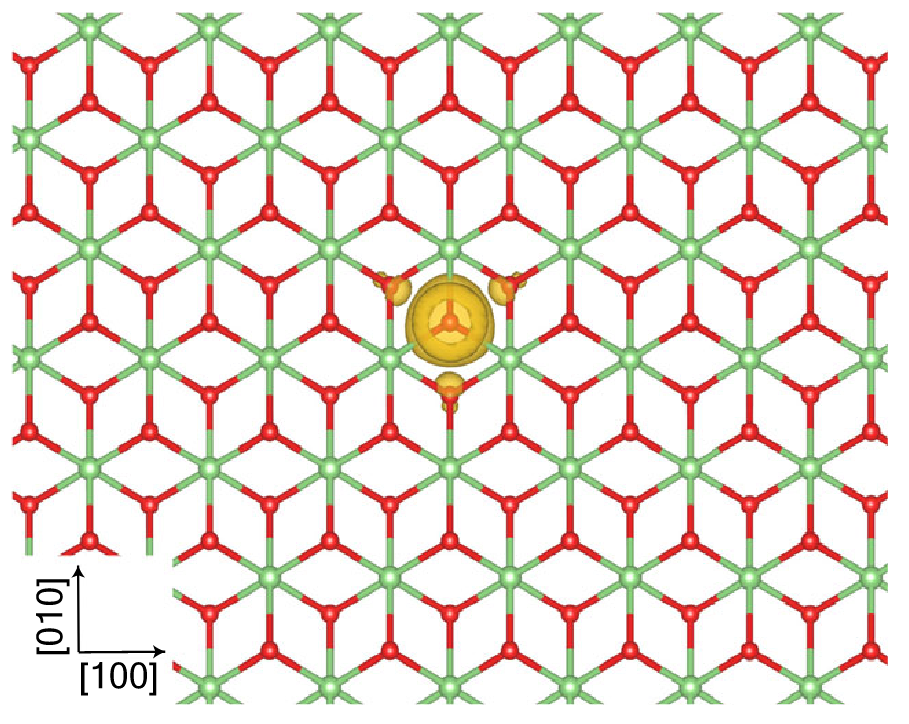
\includegraphics[width=\textwidth]{figures/small.png}
        \caption{Small polaron}
        \label{fig:small}
    \end{subfigure}
    \hfill
    \begin{subfigure}[b]{0.49\textwidth}
        \centering
        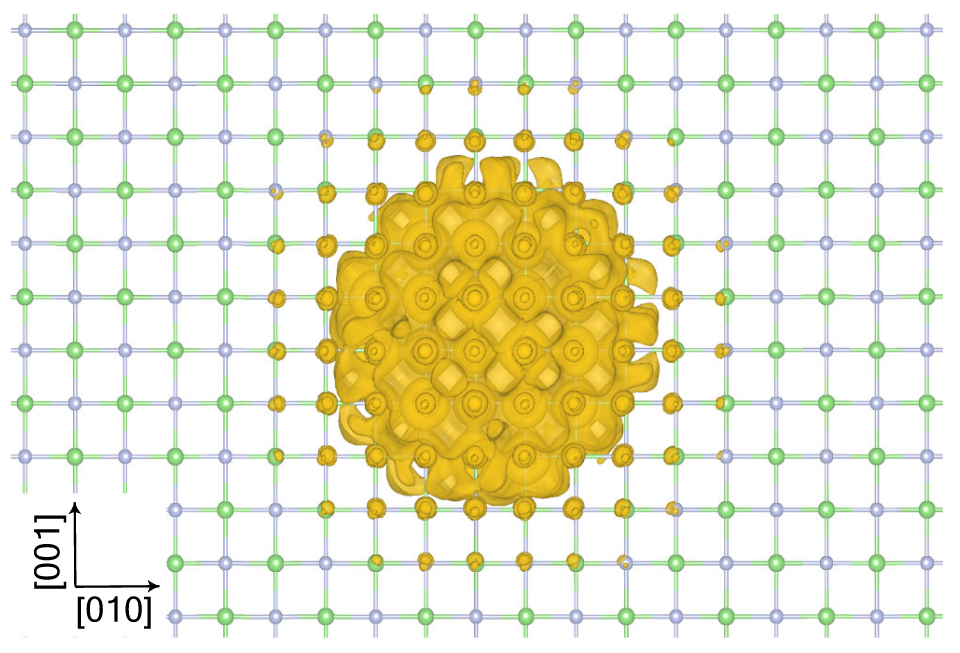
\includegraphics[width=\textwidth]{figures/large.png}
        \caption{Large polaron}
        \label{fig:large}
    \end{subfigure}
    \caption[Charge isosurfaces of a small and a large polaron]{Example of charge isosurfaces of a small and a large polaron in a 2D lattice. The images are taken from Sio et al. \cite{sio2019}}.
    \label{fig:small_large}
\end{figure}
\vfill